\section{Rezonancija}
Rezonancija je pojava koja se javlja prilikom pobude rezonancijskom frekvencijom (~\cite{dk_skripta}).
Rezonancijska frekvencija je ona frekvencija pobude za koju će dinamički koeficijent
odziva biti maksimalan (~\cite{dk_skripta}). 
\par

\subsection{Rezonancija sustava s prigušenjem}
Razmatranjem krivulja frekvencijskih funkcija odziva sa slike 
\ref{fig:rd-rv-ra}, možemo uočiti da jedino maksimumi krivulja $R_v$ padaju na 
vertikalni pravac $\omega/\omega_n=1$. Isto tako, vidljivo je da maksimalni $R_d$
pada ulijevo od navedenog pravca a maksimalni $R_a$ udesno. To znači da će se 
rezonancijske frekvencije dinamičkih faktora ($R_d$, $R_v$ i $R_a$) međusobno razlikovati 
te da će rezonancijske frekvencije dinamičkih faktora $R_d$ i $R_a$ biti različite od
prirodne frekvencije sustava.

Rezonancijske frekvencije za pojedini spektar možemo odrediti deriviranjem frekvencijske 
funkcije odziva po $\omega/\omega_n$ te izjednačavanjem prve derivacije s
nulom (~\cite{chopra2011}).
\[
    R_d = \frac{1}{\sqrt{(1-(\omega/\omega_n)^2) + (2\zeta(\omega/\omega_n))^2}}
\]
Uvodi se supstitucija $x=\omega/\omega_n$
\[
    R_d = \frac{1}{\sqrt{(1-x^2)+(2\zeta x)^2}}
\]
Deriviranjem po x dobijemo:
\[
    \frac{dR_d}{dx}=-\frac{2x^3+(4\zeta^2-2)x}{\sqrt{((1-x^2)^2+(2\zeta x)^2)^3}}
\]
Lokalni ekstrem (maksimum) dobijemo izjednačavanjem prve derivacije s nulom,
odnosno:
\[
    -\frac{2x^3+(4\zeta^2-2)x}{\sqrt{((1-x^2)^2+(2\zeta x)^2)^3}} = 0
\]
Da bi razlomak bio jednak nula izraz u brojniku mora biti jednak nula.
Izjednačavanjem brojnika s nulom dobijemo slijedeću jednadžbu:
\begin{equation}\label{eq:rv_proracun}
    2x^3 + (4\zeta^2 -2)x = 0
\end{equation}
Prvo (trivijalno) rješenje je $x=0$. Daljnim raspisom jednadžbe \eqref{eq:rv_proracun},
dobijemo slijedeću kvadratnu jednadžbu iz koje se dobije netrivijalno rješenje:
\[
    \begin{aligned}
        x^2 &= 1-2\zeta^2\\
        x &= \sqrt{1-2\zeta^2} \quad \text{ uz } \zeta < \frac{1}{\sqrt{2}}
    \end{aligned}
\]
Uvrštavanjem $\omega/\omega_n$ dobijemo izraz za rezonancijsku frekvenciju pomaka:
\begin{equation}\label{eq:rezonantna_frekvencija_pomak}
    \frac{\omega}{\omega_n}=\sqrt{1-2\zeta^2}
\end{equation}
Analogno tome dobiju se izrazi za rezonancijske frekvencije brzine i ubrzanja.
\begin{align}
    \text{Rezonancijska frekvencija pomaka}\quad & \frac{\omega}{\omega_n} = \sqrt{1-\zeta^2}\label{eq:rd_rezonanca}\\
    \text{Rezonancijska frekvencija brzine}\quad & \frac{\omega}{\omega_n} = 1 \label{eq:rv_rezonanca}\\
    \text{Rezonancijska frekvencija ubrzanja}\quad & \frac{\omega}{\omega_n} = \frac{1}{\sqrt{1-2\zeta^2}}\label{eq:ra_rezonanca}
\end{align}

Maksimalni dinamički faktori (dinamički faktori za rezonancijske frekvencije) glase
(iz (~\cite{chopra2011})):
\begin{align}
    \text{Maksimalni dinamički faktor pomaka}\quad & R_d = \frac{1}{2\zeta\sqrt{1-\zeta^2}}\\
    \text{Maksimalni dinamički faktor brzine}\quad & R_v = \frac{1}{2\zeta}\\
    \text{Maksimalni dinamički faktor ubrzanja}\quad & R_a = \frac{1}{2\zeta{1-\zeta^2}}
\end{align}

Zbog jednostavnosti, karakteristike odziva prigušenog sustava s jednim stupnjem
slobode u rezonanciji, razmotriti ćemo za slučaj $\omega = \omega_n$ uz
homogene početne uvjete. Iako se rezonancijska frekvencija pomaka ne podudara s 
prirodnom frekvencijom sustava, navedene vrijednosti su vrlo bliske za mali $\zeta$ (~\cite{chopra2011}). 
Vremenska funkcija pomaka prigušenog sustava prikazana jednadžbom \eqref{eq:inverz_treci_korak}

Uz homogene početne uvjete i za $\omega=\omega_n$, koeficijenti $A,B,C,\text{ i }D$
glase:
\begin{align}
    C &= 0 \label{eq:rez_koef_C}\\
    D &= -\frac{(u_{st})_0}{2\zeta}\label{eq:rez_koef_D}\\
    A &= -D = \frac{(u_{st})_0}{2\zeta}\label{eq:rez_koef_A}\\
    B &= -\frac{D\sigma}{\omega_D}-\frac{C\omega}{\omega_D}=
          \frac{(u_{st})_0}{2\sqrt{1-\zeta^2}}\label{eq:rez_koef_B}
\end{align}
Uvrštavanjem \eqref{eq:rez_koef_A}, \eqref{eq:rez_koef_B}, \eqref{eq:rez_koef_C} i \eqref{eq:koef_D}
u \eqref{eq:inverz_treci_korak} te sređivanjem dobijemo:
\begin{equation}\label{eq:rezonancaPrigušenoPomak}
    u(t)=\frac{(u_{st})_0}{2\zeta}\left[
        e^{-\sigma t} \left(
            \cos(\omega_D t)+\frac{\zeta}{\sqrt{1-\zeta^2}}\sin(\omega_D t)
            \right)
        -\cos(\omega_n t)
        \right]
\end{equation}
Iz navedene jednadžbe proizlazi da je amplituda odziva ograničena na
vrijednost:\footnote{Uočimo da je odziv sustava kontroliran prigušenjem (jednadžba \eqref{eq:frf_rezonanca})}

\begin{equation}\label{eq:rezonanca_amplituda}
    u_0=\frac{(u_{st})_0}{2\zeta}
\end{equation}
Za malu vrijednost $\zeta$, vrijedi $\omega_n\approx\omega_D$ te je član
uz $\sin(\omega_Dt) \text{ približno } 0$. Stoga jednadžba pod \eqref{eq:rezonancaPrigušenoPomak}
postaje:
\begin{equation}\label{eq:rezonancaOdzivAproksimacija}
    u(t)\simeq\underbrace{
        \frac{(u_{st})_0}{2\zeta}[(e^{-\sigma t}-1)
        }_{\text{Krivulja ovojnice}}
        \cos(\omega_nt)]
\end{equation}

Iz jednadžbe \eqref{eq:rezonancaOdzivAproksimacija} može se zaključiti da i za
slučaj rezonancije postoji prolazni i prisilni dio odziva, a ukupni odziv je razlika
između prolaznog i prisilnog djela. 
Prolazni dio odziva opisan je jednadžbom
\[
    e^{-\sigma t} \cos(\omega_n t)
\]
a prisilni:
\[
    \cos(\omega_n t)
\]
Za $t=0$ prolazni dio je maksimalan te je ukupni odziv jednak nuli. U ovisnosti o
vremenu, prolazni dio se smanjuje eksponencijalno prema zakonu $e^{-\sigma t}$. Kako
se prolazni dio smanjuje a prisilni ostaje isti ($(u_{st})_0/2\zeta$) tako raste
njihova razlika. Rastom razlike dolazi do rasta amplitude odziva, te isčezavanjem
prolaznog dijela preostaje samo prisilni te se dostiže maksimalna amplituda koja je
jednaka ($(u_{st})_0/2\zeta$). Bitno je za naglasiti da u teoretskom modelu
prolazni dio odziva isčezava tek za $t=\infty$, tj. asimptotski se približava nuli,
ali u realnosti prolazni dio odziva je zanemariv nakon određenog vremena. Shematski
prikaz dostizanja prisilnog stanja prikazan je na slijedećoj slici:
\begin{figure}[H]
    \begin{subfigure}[c][][l]{0.45\textwidth}
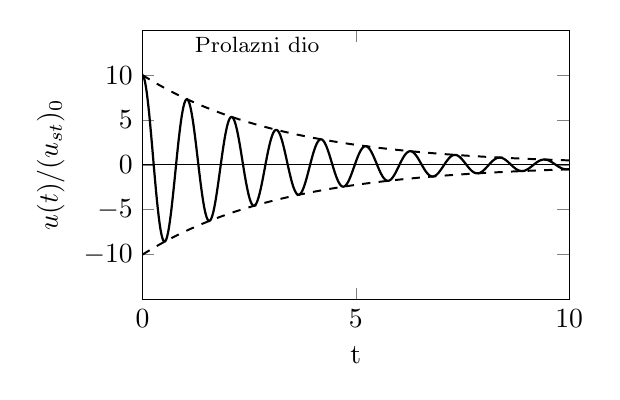
\begin{tikzpicture}
\begin{axis} [
    title={\footnotesize{Prolazni dio}},
    title style={at={(0.1,0.95)}, anchor=north west, draw=none, fill=none},
    height=5cm,
    width=7cm,
    xlabel=t,ylabel=$u(t)/(u_{st})_0$,
    ylabel near ticks, ylabel style={anchor=south},
    xmin = 0, xmax = 10,
    ymin = -15, ymax = 15,
    xtick = {0, 5, 10, 15, 20},
    ytick = {-10, -5, 0, 5, 10},
 ]
    \draw[thin] (0,0) -- (20,0);
    \addplot [
        domain=0:20,
        samples=200,
        color=black,
        dashed,line width=0.25mm,
    ] {10*exp(-0.05*6*x)};
    \addplot [
        domain=0:20,
        samples=200,
        color=black,
        dashed,line width=0.25mm,
    ] {-10*exp(-0.05*6*x)};
    \addplot [
        domain=0:20,
        samples=1000,
        color=black,
        thick,
    ] {10*exp(-0.05*6*x)*cos(6*deg(x))};
\end{axis}
\end{tikzpicture}
\end{subfigure}
\hfill
%
%
%
\begin{subfigure}[b][][r]{0.05\textwidth}
    \centering
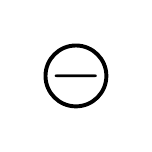
\begin{tikzpicture}[scale=5]
    \draw[thick, line width=0.5mm] (0,0) circle (2.2pt);
    \node[circle,fill=none,color=black] at (0,0) {\textbf{\Huge{$-$}}};
\end{tikzpicture}
\end{subfigure}
\hfill
%
%
%
\begin{subfigure}[c][][r]{0.45\textwidth}
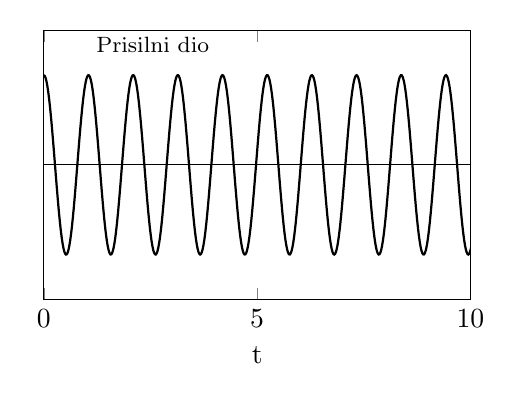
\begin{tikzpicture}
\begin{axis} [
    title={\footnotesize{Prisilni dio}},
    title style={at={(0.1,0.95)}, anchor=north west, draw=none, fill=none},
    height=5cm,
    width=7cm,
    xlabel=t,%ylabel=$u(t)/(u_{st})_0$,
%    ylabel near ticks, ylabel style={anchor=south},
    xmin = 0, xmax = 10,
    ymin = -15, ymax = 15,
    xtick = {0, 5, 10, 15, 20},
%    ytick = {-10, -5, 0, 5, 10},
    ytick=\empty,
 ]
    \draw[thin] (0,0) -- (20,0);
    \addplot [
        domain=0:20,
        samples=1000,
        color=black,
        thick,
    ] {10*cos(6*deg(x))};
\end{axis}
\end{tikzpicture}
\end{subfigure}
\vfill
%
%
%
\begin{subfigure}[b][3pt][c]{1\textwidth}
    \centering
    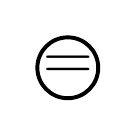
\begin{tikzpicture}[scale=5]
        \draw[thick, line width=0.5mm] (0,0) circle (2.2pt); 
        \node[circle,fill=none,color=black] at (0,0) {\textbf{\Huge{$=$}}};
    \end{tikzpicture}
\end{subfigure}
\vfill
%
%
%
\begin{subfigure}[t][][c]{1\textwidth}
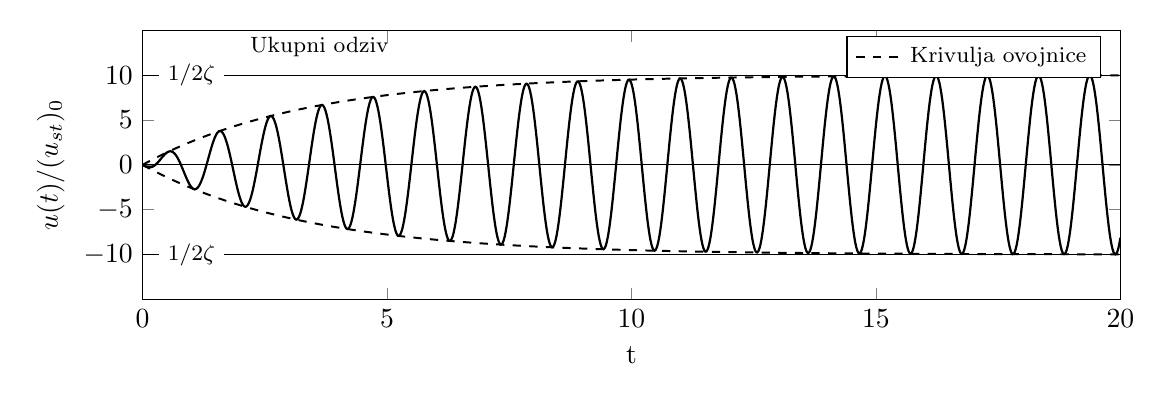
\begin{tikzpicture}
\begin{axis} [
    title={\footnotesize{Ukupni odziv}},
    title style={at={(0.1,0.95)}, anchor=north west, draw=none, fill=none},
    height=5cm,
    width=14cm,
    xlabel=t,ylabel=$u(t)/(u_{st})_0$,
    ylabel near ticks, ylabel style={anchor=south},
    xmin = 0, xmax = 20,
    ymin = -15, ymax = 15,
    xtick = {0, 5, 10, 15, 20},
    ytick = {-10, -5, 0, 5, 10},
 ]
    \draw[thin] (0,0) -- (20,0);

    \addplot [
        domain=0:20,
        samples=200,
        color=black,
        dashed,line width=0.25mm,
    ] {10*(exp(-0.05*6*x)-1)};

    \addplot [
        domain=0:20,
        samples=200,
        color=black,
        dashed,line width=0.25mm,
    ] {-10*(exp(-0.05*6*x)-1)};

    \addlegendentry{\footnotesize{Krivulja ovojnice}}

    \addplot [
        domain=0:20,
        samples=1000,
        color=black,
        thick,
    ] {10*exp(-0.05*6*x)*cos(6*deg(x))-10*cos(6*deg(x))};
%    \addlegendentry{\footnotesize{Ukupni odziv}}


    
    \draw[thin] (0,10) -- (20,10);
    \node[rectangle, fill=white] at (1,10) {\footnotesize{$1/2\zeta$}};
    \draw[thin] (0,-10) -- (20, -10);
    \node[rectangle, fill=white] at (1,-10) {\footnotesize{$1/2\zeta$}};

    \end{axis}
\end{tikzpicture}
\end{subfigure}

 
    \caption{Odziv prigušenog sustava na pobudu rezonantnom frekvencijom}
    \label{fig:rezonanca-priguseno}
\end{figure}

O prigušenju u rezonanciji ovise slijedeći parametari odziva:
\begin{itemize}
    \item brzina dostizanje ustaljenog stanja (maksimalne amplitude) - brzina dostizanja 
        ustaljenog stanja raste s prigušenjem (veće prigušenje $\to$ strmija krivulja
        ovojnice $\to$ brže dostizanje ustaljenog stanja).

    \item vrijednost maksimalne amplitude - obrnuto proporcionalna od vrijednosti
        prigušenja, definirana izrazom \eqref{eq:rezonanca_amplituda}
        (veće prigušenje, manja maksimalna amplituda, vidljivo i u frekvencijskim
        funkcijama odziva).
\end{itemize}

Određivanje broja titraja koji je potreban za dostizanje ustaljenog stanja vrši
se pomoću funkcije koja opisuje krivulju ovojnice. Pretpostavka je da ekstrem
nastupa nakon $j$ titraja ($j$ je prirodni broj), a vrijeme nastupa minimuma je
$t=2\pi j/\omega$. 
\begin{equation}\label{eq:prirastEkstremaPriguseno}
    u\left(\frac{2\pi j}{\omega_n}\right) \approx
        u_0(e^{-\zeta\omega_n\frac{2\pi j}{\omega_n}}-1)\cos\left(\omega_n\frac{2\pi
        j}{\omega_n}\right)
\end{equation}
gdje je:
\begin{table}[H]
    \begin{tabular}{c c}
        $j$ & redni broj titraja\\
        $u_0=(u_{st})_0/2\zeta$ & maksimalna amplituda\\
    \end{tabular}
\end{table}
Kako se radi o ekstremnoj vrijednosti, funkcija kosinus iznosi $\pm 1$ pa jednadžba
pod \eqref{eq:prirastEkstremaPriguseno} glasi:
\begin{equation}\label{eq:MiniMaxPriguseno}
     u\left(\frac{2\pi j}{\omega_n}\right) = u_j = 
        \pm u_0(e^{-2\pi\zeta j}-1)
\end{equation}

Za maksimume jednadžba pod \eqref{eq:MiniMaxPriguseno} postaje
\begin{equation}
    |u_j| = -u_0(e^{-2\pi\zeta j} -1) = u_0(1-e^{-2\pi\zeta j})
\end{equation}

Za relativne vrijednosti\footnote{Postotci od maksimalne amplitude}:
\begin{equation}
    u[j] = \frac{|u_j|}{u_0}=1-e^{-2j\zeta\pi}
\end{equation}
Izraz ima smisla samo za diskretne vrijednosti argumenta $j$, odnosno za $j \in
\mathbb{N}$.

\par
\begin{figure}[H]
    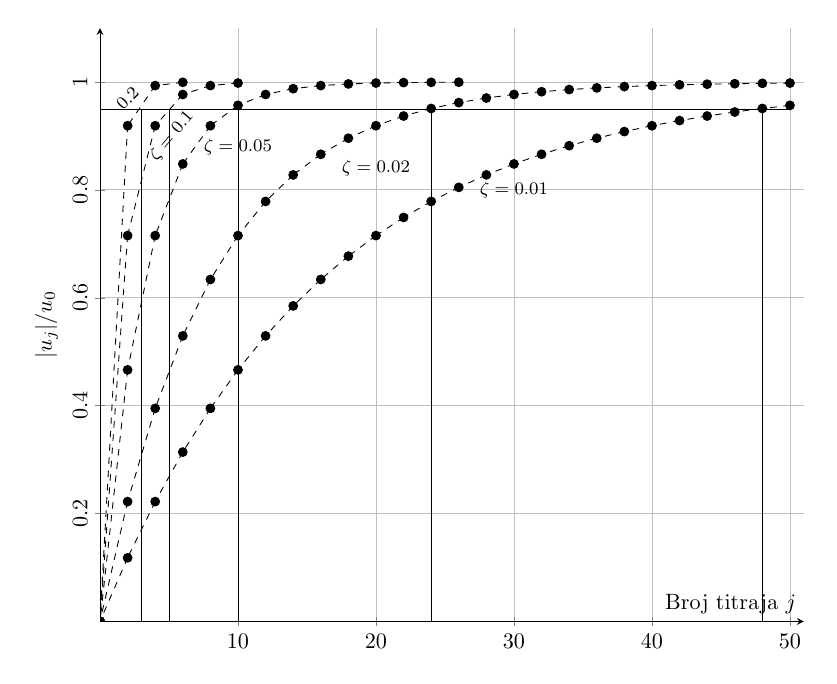
\begin{tikzpicture}[scale=0.8]
    \begin{axis} [
        height=11cm,
        axis lines=center,
        xlabel=Broj titraja $j$,
        ylabel={$|u_j|/u_0$},
        ylabel near ticks, ylabel style={anchor=south},
        xmin=0, xmax=51,
        ymin=0, ymax=1.1,
        xtick={0,10,20,30,40,50},
        ytick={0.2,0.4,0.6,0.8,1}, yticklabel style={rotate=90},
        grid=both,
    ]

        %zeta = 0.2
        \pgfplotsinvokeforeach{0, 2, 4, 6}
        {
            \filldraw( #1,{1 - exp(-2*pi*0.2*#1}) circle[radius=2pt, fill=black];
            \draw[dashed]( #1,{1 - exp(-2*pi*0.2*#1}) -- ( {#1-2}, {1-exp(-2*pi*0.2*(#1-2)});
        }

        %zeta = 0.1
        \pgfplotsinvokeforeach{0, 2, 4, ..., 10}
        {
            \filldraw( #1,{1 - exp(-2*pi*0.1*#1}) circle[radius=2pt, fill=black];
            \draw[dashed]( #1,{1 - exp(-2*pi*0.1*#1}) -- ( {#1-2}, {1-exp(-2*pi*0.1*(#1-2)});
        }

        %zeta = 0.05
        \pgfplotsinvokeforeach{0, 2, 4, ..., 26}
        {
            \filldraw( #1,{1 - exp(-2*pi*0.05*#1}) circle[radius=2pt, fill=black];
            \draw[dashed]( #1,{1 - exp(-2*pi*0.05*#1}) -- ( {#1-2}, {1-exp(-2*pi*0.05*(#1-2)});
        }

        %zeta = 0.02
        \pgfplotsinvokeforeach{0, 2, 4, ..., 50}
        {
            \filldraw( #1,{1 - exp(-2*pi*0.02*#1}) circle[radius=2pt, fill=black];
            \draw[dashed]( #1,{1 - exp(-2*pi*0.02*#1}) -- ( {#1-2}, {1-exp(-2*pi*0.02*(#1-2)});
        }

        %zeta = 0.01
        \pgfplotsinvokeforeach{0, 2, 4, ..., 50}
        {
            \filldraw( #1,{1 - exp(-2*pi*0.01*#1}) circle[radius=2pt, fill=black];
            \draw[dashed]( #1,{1 - exp(-2*pi*0.01*#1}) -- ( {#1-2}, {1-exp(-2*pi*0.01*(#1-2)});
        }

        %oznake
        \node at (30,0.80) {\footnotesize{$\zeta=0.01$}};
        \node at (20,0.84) {\footnotesize{$\zeta=0.02$}};
        \node at (10,0.88) {\footnotesize{$\zeta=0.05$}};
        \node[rotate=50] at (5.2, 0.9) {\footnotesize{$\zeta=0.1$}};
        \node[rotate=45] at (2, 0.97) {\footnotesize{$0.2$}};

        %ocitanja
        \draw[thin] (0,0.95) -- (50,0.95);
        %za 0.01
        \draw[thin] (48,0) -- (48,0.95);
        %za 0.02
        \draw[thin] (24,0) -- (24,0.95);
        %za 0.05
        \draw[thin] (10,0) -- (10,0.95);
        %za 0.1
        \draw[thin] (5,0) -- (5,0.95);
        %za 0.2
        \draw[thin] (3,0) -- (3,0.95);
    \end{axis}
\end{tikzpicture}

    \label{fig:prirast-rezonanca-priguseno}
    \caption{Ovisnost amplitude odziva o broju titraja u rezonanciji}
\end{figure}

\begin{table}[H]
    \caption{Potreban broj titraja do ustaljenog stanja}
    \label{table:prirast-rezonanca-priguseno}
    \begin{tabular}{|*{7}{c|}} % sedam stupaca; centriraj element
        \hline
        $\zeta$ & 0,01 & 0,02 & 0,05 & 0,1 & 0,2\\
        \hline
        $j$ & 48 & 24 & 10 & 5 & 3\\
        \hline
    \end{tabular}
\end{table}

Uočimo da je uz slabije prigušenje potrebno više titraja za dostizanje ustaljenog
stanja odnosno maksimalne amplitude. Očitanja vrijednosti sa grafa prikazana su u
\ref{table:prirast-rezonanca-priguseno}.



